\documentclass{article}

\usepackage[square,sort,comma,numbers]{natbib}
\usepackage{../tex_resources/ocencfd}
\usepackage{amssymb}
\usepackage{subcaption}
\usepackage{caption}
\usepackage{graphicx}
\usepackage{hyperref}
\usepackage{amsmath,amsfonts,amssymb}
\usepackage{tabularx}
\usepackage{amsmath}
\usepackage{bm}
\usepackage{mwe}
\usepackage{placeins}
\usepackage{tikz}

%%%%%%%%%% BEGIN Comment out for publication %%%%%%%%%%
% For publication, comment out the drawio package and uncomment the \newcommand line
\makeatletter
\def\input@path{{../tex_resources/}}
\makeatother
\usepackage{drawio}
%%%%%%%%%% END Comment out for publication %%%%%%%%%%

%%%%%%%%%% BEGIN Uncomment for publication %%%%%%%%%%
% \newcommand{\includediagram}[2][]{\includegraphics[#1]{#2}}
%%%%%%%%%% END Uncomment for publication %%%%%%%%%%

\usetikzlibrary{positioning, shapes.geometric, arrows.meta}

\begin{document}


\section{Include TikZ Graph}

This graph is an idea I was toying around with, but I have not tried it yet.

\begin{figure}[ht]
\centering


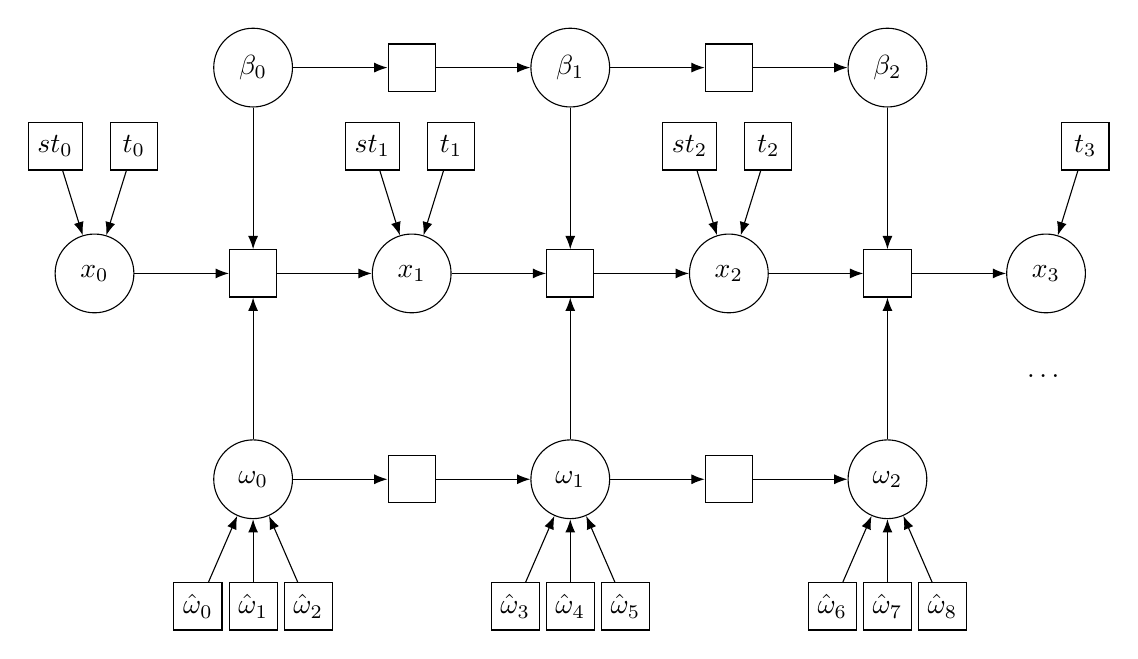
\begin{tikzpicture}[
    node distance=1.8cm and 1.2cm, % Vertical and horizontal spacing
    block/.style={draw, rectangle, minimum height=0.6cm, minimum width=0.6cm, align=center},
    circle_node/.style={draw, circle, minimum size=1.0cm, inner sep=0pt, align=center},
    empty_node/.style={minimum size=0.8cm} % For spacing, if needed
]

%%%%% Main Chain of Nodes
\node[circle_node] (x0) {$x_0$};
\node[block,        right=of x0] (f0) {};
\node[circle_node,  right=of f0] (x1) {$x_1$};
\node[block,        right=of x1] (f1) {};
\node[circle_node,  right=of f1] (x2) {$x_2$};
\node[block,        right=of x2] (f2) {};
\node[circle_node,  right=of f2] (x3) {$x_3$};


%  Star tracker measurements
\node[block, above=of x0, xshift=-0.5cm, yshift=-1cm] (zst0) {$st_0$};
\node[block, above=of x1, xshift=-0.5cm, yshift=-1cm] (zst1) {$st_1$};
\node[block, above=of x2, xshift=-0.5cm, yshift=-1cm] (zst2) {$st_2$};


%  Timestamps
\node[block, above=of x0, xshift=0.5cm, yshift=-1cm] (zt0) {$t_0$};
\node[block, above=of x1, xshift=0.5cm, yshift=-1cm] (zt1) {$t_1$};
\node[block, above=of x2, xshift=0.5cm, yshift=-1cm] (zt2) {$t_2$};
\node[block, above=of x3, xshift=0.5cm, yshift=-1cm] (zt3) {$t_3$};


% Angular velocity Chain
\node[circle_node,  below=of f0]  (w0) {$\omega_0$};
\node[block,        right=of w0]  (rb0) {};
\node[circle_node,  right=of rb0]  (w1) {$\omega_1$};
\node[block,        right=of w1]  (rb1) {};
\node[circle_node,  right=of rb1]  (w2) {$\omega_2$};

% \node[block,        left=of w0]   (PB) {Prior};

% Angular velocity bias Chain
\node[circle_node,  above=of f0]  (b0) {$\beta_0$};
\node[block,        right=of b0]  (brb0) {};
\node[circle_node,  right=of brb0]  (b1) {$\beta_1$};
\node[block,        right=of b1]  (brb1) {};
\node[circle_node,  right=of brb1]  (b2) {$\beta_2$};

% Angular velocity measurements
\node[block, below=of w0, xshift=-0.7cm, yshift=1cm] (zw0) {$\hat{\omega}_0$};
\node[block, below=of w0, xshift= 0.0cm, yshift=1cm] (zw1) {$\hat{\omega}_1$};
\node[block, below=of w0, xshift= 0.7cm, yshift=1cm] (zw2) {$\hat{\omega}_2$};

\node[block, below=of w1, xshift=-0.7cm, yshift=1cm] (zw3) {$\hat{\omega}_3$};
\node[block, below=of w1, xshift= 0.0cm, yshift=1cm] (zw4) {$\hat{\omega}_4$};
\node[block, below=of w1, xshift= 0.7cm, yshift=1cm] (zw5) {$\hat{\omega}_5$};

\node[block, below=of w2, xshift=-0.7cm, yshift=1cm] (zw6) {$\hat{\omega}_6$};
\node[block, below=of w2, xshift= 0.0cm, yshift=1cm] (zw7) {$\hat{\omega}_7$};
\node[block, below=of w2, xshift= 0.7cm, yshift=1cm] (zw8) {$\hat{\omega}_8$};


%  Draw arrows between nodes

\draw[-Latex] (x0) -- (f0);
\draw[-Latex] (f0) -- (x1);
\draw[-Latex] (x1) -- (f1);
\draw[-Latex] (f1) -- (x2);
\draw[-Latex] (x2) -- (f2);
\draw[-Latex] (f2) -- (x3);

\draw[-Latex] (w0) -- (f0);
\draw[-Latex] (w1) -- (f1);
\draw[-Latex] (w2) -- (f2);

\draw[-Latex] (b0) -- (f0);
\draw[-Latex] (b1) -- (f1);
\draw[-Latex] (b2) -- (f2);


% \draw[-Latex] (PB) -- (w0);

\draw[-Latex] (zst0) -- (x0);
\draw[-Latex] (zst1) -- (x1);
\draw[-Latex] (zst2) -- (x2);

\draw[-Latex] (zt0) -- (x0);
\draw[-Latex] (zt1) -- (x1);
\draw[-Latex] (zt2) -- (x2);
\draw[-Latex] (zt3) -- (x3);

\draw[-Latex] (zw0) -- (w0);
\draw[-Latex] (zw1) -- (w0);
\draw[-Latex] (zw2) -- (w0);

\draw[-Latex] (zw3) -- (w1);
\draw[-Latex] (zw4) -- (w1);
\draw[-Latex] (zw5) -- (w1);

\draw[-Latex] (zw6) -- (w2);
\draw[-Latex] (zw7) -- (w2);
\draw[-Latex] (zw8) -- (w2);


\draw[-Latex] (w0) -- (rb0);
\draw[-Latex] (rb0) -- (w1);
\draw[-Latex] (w1) -- (rb1);
\draw[-Latex] (rb1) -- (w2);

\draw[-Latex] (b0) -- (brb0);
\draw[-Latex] (brb0) -- (b1);
\draw[-Latex] (b1) -- (brb1);
\draw[-Latex] (brb1) -- (b2);



\path (x3) -- node[auto=false, xshift=1cm]{\ldots} (w2);

\end{tikzpicture}



\caption{Factor Graph with Timestamp Estimation}
\label{fig:factor_graph}
\end{figure}


\section{Include DrawIO Graph}

This graph is in ../drawio/factor_graph_1.drawio. If the graph file is updated, compile this document again (ctrl+s or hit play) to see the changes. Converting from .drawio to .pdf is done automatically if the drawio file changes, so it takes a bit longer to compile the first time after a change.

If you decide to publish this document, comment out the drawio package and uncomment the \verb|\newcommand| line above. This will include the .pdf file directly instead of converting from .drawio to .pdf on the fly. When submitting, make sure to include the .pdf files.

\begin{figure}[ht]
\centering
\includediagram{../drawio/factor_graph_1}
\caption{Factor Graph with Timestamp Estimation}
\label{fig:factor_graph_1}
\end{figure}


\end{document} 
